\documentclass[tikz,12pt,margin=0px]{article}

\usepackage[a4paper, margin=1in]{geometry}
\usepackage[export]{adjustbox}
\usepackage[magyar]{babel}
\usepackage[normalem]{ulem}
\usepackage[utf8]{inputenc}
\usepackage{amsmath}
\usepackage{amssymb}
\usepackage{enumitem}
\usepackage{fancyhdr}
\usepackage{fontawesome}
\usepackage{listings}
\usepackage{pgfplotstable}
\usepackage{setspace}
\usepackage[utf8]{inputenc}
\usepackage{amsmath}
\usepackage{amssymb}
\usepackage{collectbox}
\usepackage{comment}
\usepackage{float}
\usepackage{svg}
\usepackage{tikz}
%\usepackage{titlesec}

\newcommand\ddfrac[2]{\frac{\displaystyle #1}{\displaystyle #2}}

 \geometry{
 a4paper,
 total={170mm,257mm},
 left=20mm,
 right=20mm,
 top=20mm,
 bottom=20mm
 }

\setlist[itemize,1]{label=$\bullet$}
\setlist[itemize,2]{label=$\circ$}
\setlist[itemize,3]{label=$\centerdot$}
\setlist[itemize,4]{label=$\cdot$}

\pagestyle{fancy}

\newcommand\blfootnote[1]{%
  \begingroup
  \renewcommand\thefootnote{}\footnote{#1}%
  \addtocounter{footnote}{-1}%
  \endgroup
}

\renewcommand{\figurename}{ábra}
\newenvironment{tetel}[1]{\paragraph{#1 \\}}{}

\newcommand{\N}{\mathbb{N}}
\newcommand{\Z}{\mathbb{Z}}
\newcommand{\R}{\mathbb{R}}
\newcommand{\Q}{\mathbb{Q}}
\newcommand{\C}{\mathbb{C}}

\makeatletter
\renewcommand\paragraph{%
	\@startsection{paragraph}{4}{0mm}%
	{-\baselineskip}%
	{.5\baselineskip}%
	{\normalfont\normalsize\bfseries}}
\makeatother

% A dokument itt kezdődik

\useunder{\uline}{\ul}{}
\fancyhead{}
\cfoot{1. tétel | \thepage. oldal}

\renewcommand{\headrulewidth}{0pt}
\renewcommand{\footrulewidth}{0.4pt}

\begin{document}
%    \pagecolor{black!40}
%    \color{white}
    \thispagestyle{fancy}
    \hyphenation{oddword}
    \uchyph=0

    {\Large\bfseries\noindent 1. Függvények határértéke, folytonossága\\}

    \noindent Jelölje a továbbiakban $\overline{\mathbb{R}} = \mathbb{R} \cup \{+\infty, -\infty\}$ (bővített számegyenes)\\

	\noindent \textbf{Környezet}: Legyen $a \in \mathbb{R}$, és $\delta \in \mathbb{R}^{+}$, ekkor a
    \begin{itemize}
        \item \textbf{\small \emph{Kétoldali környezet}}: $K_{\delta}(a)\ =\ \Big\{x \in \mathbb{R}\ \Big|\ \emph{d}(x,a) = |x-a|\ <\ \delta \Big\}\ =\ (a - \delta,\ a + \delta)$
        \item \textbf{\small \emph{Bal oldali környezet}}: $K_{\delta}(a-0)\ =\ K(a-0)\ =\ (a - \delta,\ a)$
        \item \textbf{\small \emph{Jobb oldali környezet}}: $K_{\delta}(a+0)\ =\ K(a+0)\ =\ (a,\ a + \delta)$
        \item Ha $a \in \overline{\mathbb{R}}$ és $c \in \mathbb{R}$, akkor \emph{kiterjesztett környezet}ről beszélünk, és
        \begin{align*}
            K_{c}(+\infty) = \left(c, +\infty \right) = \Big\{ x \in \mathbb{R}\ \Big|\ c < x \Big\}\\
            K_{c}(-\infty) = \left(-\infty, c \right) = \Big\{ x \in \mathbb{R}\ \Big|\ x < c \Big\}
        \end{align*}
    \end{itemize}

    \paragraph*{Belső pont}

    \noindent Legyen $A \subset \mathbb{R}$ tetszőleges halmaz és $a \in \mathbb{R}$. Az $a$ \textbf{belső pontja} a $A$ halmaznak, ha az $a$-nak van olyan $\delta > 0$ sugarú környezete, amely részhalmaza az $A$-nak ($K_{\delta}(a) \subset A)$.\\
    \noindent \emph{Jelölése}: \textbf{int A} (az A halmaz belső pontjainak halmaza).
	
	\paragraph*{Torlódási pont}
    Az $a \in \overline{\mathbb{R}}$, az $\emptyset \neq H \subset \mathbb{R}$ halmaz \textbf{torlódási pontja}, ha $\forall \delta > 0 : K_{\delta}(a) \cap H$ végtelen halmaz, azaz az $a$ pont minden környezete végtelen sok $H$-beli elemet tartalmaz.\\
    \noindent \emph{Jelölése}: $\textbf{H}\boldsymbol{'}$ (a H halmaz torlódási pontjainak halmaza).\\
	
    \noindent Megjegyzések:
    \begin{itemize}
        \item Az $a \in \mathbb{R}$ torlódási pontja az $A$-nak, ha $\forall \delta > 0: (a - \delta, a + \delta) \cap A$ végtelen halmaz.
        \item Az $a = +\infty \in \overline{\mathbb{R}}$ torlódási pontja az $A$-nak, ha $\forall \delta > 0: (\delta, +\infty) \cap A$ végtelen halmaz.
        \item Az $a = -\infty \in \overline{\mathbb{R}}$ torlódási pontja az $A$-nak, ha $\forall \delta > 0: (-\infty, -\delta) \cap A$ végtelen halmaz.\\
    \end{itemize}

    \noindent \textbf{Példa 1.} Az $\left\{\ddfrac{1}{n} \Big|\ n = 1, 2, \ldots\right\}$ egyetlen torlódási pontja a \textbf{0}.

    \begin{center}
        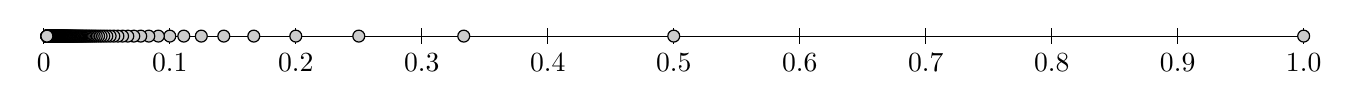
\begin{tikzpicture}
            \draw[-] (0.00,0.00) -- (16.00,00);

            \foreach \x in {0,0.1,0.2,0.3,0.4,0.5,0.6,0.7,0.8,0.9,1.0}
                \draw (\x * 16,0.1) -- (\x * 16,-0.1) node [below] {\x};

            \foreach\x [evaluate=\x as \y using 1/\x] in {1,...,400}
                \draw[red,fill={rgb:black,1;white,4},line width=.1ex,draw=black] (\y * 16,0) circle (.5ex);

        \end{tikzpicture}
    \end{center}
    \ \\
    \noindent \textbf{Példa 2.} A $\left\{(-1)^{n} \cdot \left(2 - \ddfrac{1}{n}\right) \Big|\ n = 1, 2, \ldots\right\}$ két torlódási pontja a \textbf{-2} és a \textbf{2}.

    \begin{center}
        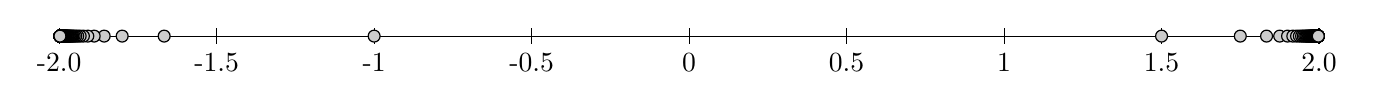
\begin{tikzpicture}
            \draw[-] (-8.00,0.00) -- (8.00,00);

            \foreach \x in {-2.0, -1.5, ..., 1.5, 2.0}
                \draw (\x * 4,0.1) -- (\x * 4,-0.1) node [below] {\x};

            \foreach\x [evaluate=\x as \y using ((-1)^\x) * (2 - 1/\x)] in {1,...,400}
                \draw[red,fill={rgb:black,1;white,4},line width=.1ex,draw=black] (\y * 4,0) circle (.5ex);
        \end{tikzpicture}
    \end{center}
    \ \\
    \noindent További példák: $\mathbb{N}' = \{+\infty\},\quad \mathbb{Q}' = \overline{\mathbb{R}},\quad \mathbb{Q}^{*'} = \overline{\mathbb{R}},\quad (0,1)' = [0,1]$.\\
\newpage

    {\footnotesize \noindent {\color{blue} \faLightbulbO\ $\triangleright$ } }
    {\footnotesize

	\noindent \textbf{Nyílt halmaz}\\

	\noindent $A$ nyílt halmaz $\iff\ \forall a \in A,\ \exists K(a): K(a) \subset A$, vagyis az $A$ halmaz minden pontja belső pont.\\
    \noindent Másképp: Adott $a,\ b \in \mathbb{R}$, ahol $a < b$. Ekkor az $a$ és $b$ számok által meghatározott nyílt intervallumon az $\left\{ x \in \mathbb{R}\ \big|\ a < x < b\right\}$ halmazt értjük. Jelölése: $\Big(a,b\Big)$ vagy $\Big]a,b\Big[$\\\\

	\noindent \textbf{Zárt halmaz}\\
	
	\noindent Komplementere nyílt halmaz.\\
    \noindent Másképp: Adott $a,\ b \in \mathbb{R}$, ahol $a < b$. Ekkor az $a$ és $b$ számok által meghatározott zárt intervallumon az $\left\{ x \in \mathbb{R}\ \big|\ a \leq x \leq b\right\}$ halmazt értjük. Jelölése: $[a,b]$\\

    \noindent Legyen $A \subset \mathbb{R},\ A \neq \emptyset$. Azt mondjuk, hogy
    \begin{itemize}
        \item $A$ \textbf{felülről korlátos} számhalmaz, ha $\exists K \in \mathbb{R}$, hogy bármely $a \in A$ esetén $a \leq K$.\\ Az ilyen $K$ szám az $A$ halmaz egyik felső korlátja.\\
    \end{itemize}

    \noindent Legyen $A \subset \mathbb{R},\ A \neq \emptyset$ \emph{felülről korlátos} halmaz. \\
    Tekintsük a $B := \Big\{K \in \mathbb{R}\ \Big|\ \text{\emph{K} felső korlátja az \emph{A} halmaznak}\Big\}$ halmazt.\\
    Legyen $\alpha \in \mathbb{R}$ a $B$ halmaz legkisebb eleme, azaz olyan szám, amelyre
    \begin{itemize}
        \item $\alpha \in B$ ($\alpha$ is \emph{felső korlátja} az $A$ halmaznak)
        \item bármely $K \in B$ felső korlátra $\alpha \leq K$. A kérdés csupán az, hogy van-e ilyen $\alpha \in \mathbb{R}$.
    \end{itemize}

    \noindent Az ilyen $\alpha \in \mathbb{R}$ számot (amely nem feltétlenül eleme az $A$ halmaznak) a halmaz \textbf{felső határának} nevezzük.
    \noindent Jelölése:
    \[
        \alpha := sup A\ \text{(„az A halmaz szuprémuma”)}
    \]

    \noindent A $supA$ két tulajdonsága:
    \begin{itemize}
        \item bármely $a \in A$ esetén $a \leq supA$
        \item bármely $\varepsilon > 0$ esetén van olyan $a' \in A$, hogy $(supA) -\varepsilon < a'$.\\
    \end{itemize}

    \noindent \textbf{Felső határ axiómája}: Minden \emph{felülről korlátos} $A \subset \mathbb{R},\ A \neq \emptyset$ halmaznak van \emph{legkisebb felső korlátja}.\\

    \noindent Legyen $A \subset \mathbb{R},\ A \neq \emptyset$. Azt mondjuk, hogy
    \begin{itemize}
        \item $A$ \textbf{alulról korlátos} számhalmaz, ha $\exists L \in \mathbb{R}$, hogy bármely $a \in A$ esetén $a \geq L$.\\ Az ilyen $L$ szám az $A$ halmaz egyik alsó korlátja.\\
    \end{itemize}

    \noindent Legyen $A \subset \mathbb{R},\ A \neq \emptyset$ \emph{alulról korlátos} halmaz. \\
    Tekintsük a $B := \Big\{L \in \mathbb{R}\ \Big|\ \text{\emph{L} alsó korlátja az \emph{A} halmaznak}\Big\}$ halmazt.\\
    Legyen $\beta \in \mathbb{R}$ a $B$ halmaz legnagyobb eleme, azaz olyan szám, amelyre
    \begin{itemize}
        \item $\beta \in B$ ($\beta$ is \emph{alsó korlátja} az $A$ halmaznak)
        \item bármely $L \in B$ alsó korlátra $\beta \leq L$.
    \end{itemize}

    \noindent Az ilyen $\beta \in \mathbb{R}$ számot (amely nem feltétlenül eleme az $A$ halmaznak) a halmaz \textbf{alsó határának} nevezzük.
    Jelölése:
    \[
        \beta := inf A\ \text{(„az A halmaz infimuma”)}
    \]

    \noindent Az $infA$ két tulajdonsága:
    \begin{itemize}
        \item bármely $a \in A$ esetén $infA \leq a$
        \item bármely $\varepsilon > 0$ esetén van olyan $a' \in A$, hogy $a' < (infA) +\varepsilon$.
    \end{itemize}

%    \noindent \textbf{Definíció}. Legyen $I \subset \mathbb{R}$. Azt mondjuk, hogy $I$ \textbf{intervallum}, ha bármely $x_{1}, x_{2} \in I,\ x1 < x2$ esetén minden olyan $x \in \mathbb{R}$, amelyre $x_1 < x < x_2$, fennáll, hogy $x \in I$.\\
    }
    \noindent {\footnotesize $\triangleleft$ \faLightbulbO }\\

    \noindent Akkor mondjuk, hogy a $\mathbb{R}$ valamely $I$ részhalmaza \textbf{kompakt}, ha $I$ \emph{korlátos} és \emph{zárt} halmaz.\\

	\section*{Függvények határértéke}
	
    \textit{Intuitívan}: Legyen $a$ egy nyílt intervallum egy pontja és tegyük fel, hogy az $f$ függvény értelmezve van ezen az intervallumon, kivéve esetleg magát az $a$ helyet.\\
     Ha az $f(x)$ függvényértékek tetszőlegesen közel kerülhetnek egy $A$ számhoz, amennyiben az $x$ értékek eléggé megközelítik az $a$-t, akkor azt mondjuk, hogy $f$ függvény az $A$ számhoz tart, miközben $x$ tart $a$-hoz.\\

    \noindent Legyen $f \in \mathbb{R} \rightarrow \mathbb{R},\ a \in D_{f}^{'} \subset \overline{\mathbb{R}}$.\\
    Az $f$ függvénynek az $a \in D_{f}^{'}$ pontban létezik határértéke az $A \in \overline{\mathbb{R}}$, ha
    \[
        \forall \varepsilon > 0\qquad \exists \delta > 0\qquad \forall x \in \Big(K_{\delta}(a)\setminus\{a\} \cap D_{f} \Big)\text{ esetén }f(x) \in K_{\varepsilon}(A)
    \]

    \begin{center}
        Jelölés: $\lim\limits_{x \to a}{f(x)} = \lim\limits_{a}{f} = A$
    \end{center}

    \paragraph*{Végesben vett véges határérték\\}

    {\footnotesize \noindent {\color{blue} \faLightbulbO\ $\triangleright$ } }

    {\footnotesize

    \noindent Legyen $f : \mathbb{R} \rightarrow \mathbb{R}$ tetszőleges függvény, $a \in \mathbb{R}$ tetszőleges szám, amelynek valamely $\delta$ sugarú lyukas környezetét $Dom(f)$ tartalmazza.  Ekkor az $f(x)$ függvénynek az $a$ pontban (végesben) van véges határértéke, ha van olyan $A \in \mathbb{R}$ valós szám, amelynek minden $\varepsilon > 0$ sugarú környezetéhez (hiba-vagy türéshatár) található az $a$ számnak egy olyan $\delta > 0$ sugarú környezete (küszöbhatár), amelynek minden $x$ eleme esetén $f(x)$ az A-nak $\varepsilon$ sugarú környezetébe esik (vagyis $f(x)$ értéke $A$-tól legfeljebb $\varepsilon$-al tér el).\\
    }
    \noindent {\footnotesize $\triangleleft$ \faLightbulbO }\\

    \noindent Legyen $f \in \mathbb{R} \rightarrow \mathbb{R},\ a \in D_{f}^{'} \subset \mathbb{R}$, ekkor
    \begin{center}
        $\lim\limits_{x \to a}^{}f = A \in \mathbb{R}$\\
        $\Updownarrow$\\
        $\forall \varepsilon > 0\qquad \exists \delta > 0\qquad \forall x \in D_{f}\quad \Big[0 < \big|x - a\big| < \delta\ : \big|f(x) - A\big| < \varepsilon\Big]$
    \end{center}

    {\footnotesize \noindent {\color{blue} \faLightbulbO\ $\triangleright$ } }
    {\footnotesize

    \noindent Ha az $f$ \emph{identikus leképezés}, azaz minden $x$-re, $f(x) = x$, akkor tetszőleges $a$ esetén
    \[
        \lim\limits_{x \to a}f(x) = \lim\limits_{x \to a}x = a
    \]

    \noindent Ha az $f$ \emph{abszolút érték függvény}, azaz minden  $x$-re $f(x) = \Big|x\Big|$, akkor tetszőleges $a$ esetén
    \[
        \lim\limits_{x \to a}f(x) = \lim\limits_{x \to a}\Big|x\Big| = \Big|a\Big|
    \]

    \noindent Ha az $f$ \emph{konstans függvény}, azaz minden  $x$-re $f(x) = k$ valamely $k$ számra, akkor tetszőleges $a$ esetén
    \[
        \lim\limits_{x \to a}f(x) = \lim\limits_{x \to a}k = k
    \]
    }
    \noindent {\footnotesize $\triangleleft$ \faLightbulbO }
\newpage
    \paragraph*{Végesben vett végtelen határérték\\}

    \noindent Legyen $f \in \mathbb{R} \rightarrow \mathbb{R},\ a \in D_{f}^{'} \subset \mathbb{R}$, ekkor\\

    \noindent \emph{Végesben vett mínusz végtelen határérték}:
    \begin{center}
        $\lim\limits_{x \to a}f = -\infty$\\
        $\Updownarrow$\\
        $\forall K \in \mathbb{R}\qquad \exists \delta > 0\qquad \forall x \in D_{f}\quad \Big[0 < \big|x - a\big| < \delta:\ f(x) \boldsymbol{<} K\Big]$
    \end{center}

    \noindent \emph{Végesben vett plusz végtelen határérték:}
    \begin{center}
        $\lim\limits_{x \to a}f = +\infty$\\
        $\Updownarrow$\\
        $\forall K \in \mathbb{R}\qquad \exists \delta > 0\qquad \forall x \in D_{f}\quad \Big[0 < \big|x - a\big| < \delta:\ f(x) \boldsymbol{>} K\Big]$
    \end{center}

%    \begin{center}
%        \begin{tikzpicture}[scale=1.0]
%          \begin{axis}[axis lines=middle,xmin=-5.0,xmax=5.0,ymin=0.0,ymax=2.0,
%            xlabel=$\scriptstyle x$,
%            ylabel=$\scriptstyle y$,
%            xtick={-5,-4,-3,-2,-1,0,1,2,3,4,5},
%            ytick={0,0.5,1.0,2.0},
%            xticklabels={-5,4,$\Big(0 - \delta$,-2,-1,0,1,2,$0 + \delta\Big)$,4,5},
%            extra x ticks={0},
%            tick label style={font=\tiny}]
%            \addplot[no marks, line width=2pt,gray,domain=-5.0:-3.1,samples=15]
%            {
%                1/(x^2)
%            };
%            \addplot[no marks, line width=2pt,blue,domain=-2.9:2.9,samples=40]
%            {
%                1/(x^2)
%            };
%            \addplot[no marks, line width=2pt,gray,domain=3.1:5.0,samples=15]
%            {
%                1/(x^2)
%            };
%            \addplot+[no marks,thick, line width=0.75pt,red,dotted] plot coordinates
%	        {
%                (-3,0) (-3,0.1)
%            };
%            \addplot+[no marks,thick, line width=0.75pt,red,dotted] plot coordinates
%	        {
%                (-3,0.15) (-3,3)
%            };
%            \addplot+[no marks,thick, line width=0.75pt,red,dotted] plot coordinates
%	        {
%                (3,0) (3,0.1)
%            };
%            \addplot+[no marks,thick, line width=0.75pt,red,dotted] plot coordinates
%	        {
%                (3,0.15) (3,3)
%            };
%            \addplot+[xcomb,no marks,thick, line width=1pt,red] plot coordinates
%            {
%                (-2.9,0.1111111) (2.9,0.1111111)
%            };
%            \addplot[only marks,mark=o,red] coordinates
%            {
%                (-3.0,0.1111111) (3.0,0.1111111)
%            };
%            \addplot[only marks,mark=*,red] coordinates { (0,0) };
%            %\node[above right, outer sep=2pt] (0.0,0.1111111) {P};
%          \end{axis}
%        \end{tikzpicture}
%        \begin{tikzpicture}[scale=1.0]
%          \begin{axis}[axis lines=middle,xmin=-2.0,xmax=2.0,ymin=0.0,ymax=3.0,
%            xlabel=$\scriptstyle x$,
%            ylabel=$\scriptstyle y$,
%            ytick={0,0.5,1,1.5,2,2.5,3.0},
%            xtick={-2,-1,0,1,2},
%            xticklabels={2,$\Big(0 - \delta$,0,$0 + \delta\Big)$,2},
%            extra x ticks={0},
%            tick label style={font=\tiny}]
%            \addplot[no marks, line width=2pt,gray,domain=-2.0:-1.0163,samples=20]
%            {
%                1/(x^2)
%            };
%            \addplot[no marks, line width=2pt,gray,domain=-2.0:-1.0163,samples=20]
%            {
%                1/(x^2)
%            };
%            \addplot[no marks, line width=2pt,blue,domain=-0.9845:-0.1,samples=16]
%            {
%                1/(x^2)
%            };
%            \addplot[no marks, line width=2pt,blue,domain=0.1:0.9845,samples=16]
%            {
%                1/(x^2)
%            };
%            \addplot[no marks, line width=2pt,gray,domain=1.0163:2.0,samples=20]
%            {
%                1/(x^2)
%            };
%            \addplot+[no marks,thick, line width=0.75pt,red,dotted] plot coordinates
%	        {
%                (-1,0) (-1,0.963)
%            };
%            \addplot+[no marks,thick, line width=0.75pt,red,dotted] plot coordinates
%	        {
%                (-1,1.037) (-1,3)
%            };
%            \addplot+[no marks,thick, line width=0.75pt,red,dotted] plot coordinates
%	        {
%                (1,0) (1,0.963)
%            };
%            \addplot+[no marks,thick, line width=0.75pt,red,dotted] plot coordinates
%	        {
%                (1,1.037) (1,3)
%            };
%            \addplot+[xcomb,no marks,thick, line width=1pt,red] plot coordinates
%            {
%                (-0.963,1.0) (0.963,1.0)
%            };
%            \addplot[only marks,mark=o,red] coordinates
%            {
%                (-1.0,1.0) (1.0,1.0)
%            };
%            \addplot[only marks,mark=*,red] coordinates { (0,0) };
%            %\node[above right, outer sep=2pt] (0.0,1.0) {P};
%          \end{axis}
%        \end{tikzpicture}
%    \end{center}

    \paragraph*{Végtelenben vett véges határérték\\}

    \noindent \emph{Mínusz végtelenben vett véges határérték}:
    \begin{center}
        $\lim\limits_{x \to \boldsymbol{-\infty}}^{}f = \textbf{A}$\\
        $\Updownarrow$\\
        $\forall \varepsilon > 0\qquad \exists \omega \in \mathbb{R}\ \text{(küszöbszám)}\qquad \forall x \in D_{f}\quad \Big[x \boldsymbol{<} \omega:\ \big|f(x) - A\big| < \varepsilon\Big]$
    \end{center}
    \noindent \emph{Plusz végtelenben vett véges határérték}:
    \begin{center}
        $\lim\limits_{x \to \boldsymbol{+\infty}}^{}f = \textbf{A}$\\
        $\Updownarrow$\\
        $\forall \varepsilon > 0\qquad \exists \omega \in \mathbb{R}\ \text{(küszöbszám)}\qquad \forall x \in D_{f}\quad \Big[x \boldsymbol{>} \omega:\ \big|f(x) - A\big| < \varepsilon\Big]$
    \end{center}

    \noindent \emph{Példa}: $\lim\limits_{x \to +\infty} 2 + \ddfrac{1}{x^{2}} = 2$. \\

    \noindent Akárhogy választjuk az $\varepsilon > 0$ számot, lesz olyan $K > 0$, hogy ettől az értéktől kezdve minden $x$-re, a függvényértékek $f(x)$ $2$-től vett távolsága kisebb, mint $\varepsilon$.

    \begin{center}
        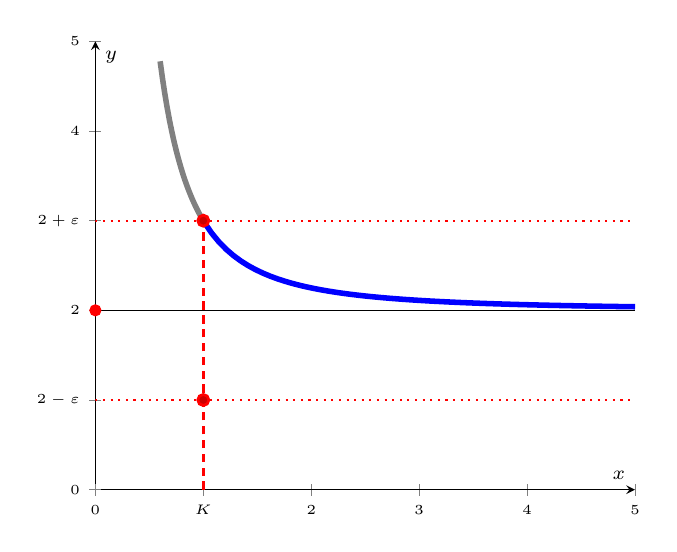
\begin{tikzpicture}[scale=1.0]
          \begin{axis}[axis lines=center,xmin=0.0,xmax=5.0,ymin=0.0,ymax=5.0,
            xlabel=$\scriptstyle x$,
            ylabel=$\scriptstyle y$,
            xtick={0,1,2,3,4,5},
            ytick={0,1,2,3,4,5},
            xticklabels={0,$K$,2,3,4,5},
            yticklabels={0,$2 - \varepsilon$,2,$2 + \varepsilon$,4,5},
            extra x ticks={0.0},
            extra y ticks={0.0},
            tick label style={font=\tiny}]
            \addplot[no marks, line width=2pt,gray,domain=0.6:1.0,samples=20] {2 + 1/(x^2)};
            \addplot[no marks, line width=2pt,blue,domain=1.01:5.0,samples=60] {2 + 1/(x^2)};
            \addplot[only marks,mark=*,red] coordinates { (0,2) };
            \addplot+[xcomb,no marks,thick, line width=0.3pt,black] plot coordinates
	           {(0,2) (5,2)};
            \addplot+[xcomb,no marks,dotted, line width=0.75pt,red] plot coordinates
                {
                    (1,3) (5,3)
                    (1,1) (5,1)
                };
            \addplot+[ycomb, line width=1pt,red] plot coordinates
	           {(1,1) (1,3)};
          \end{axis}
        \end{tikzpicture}
        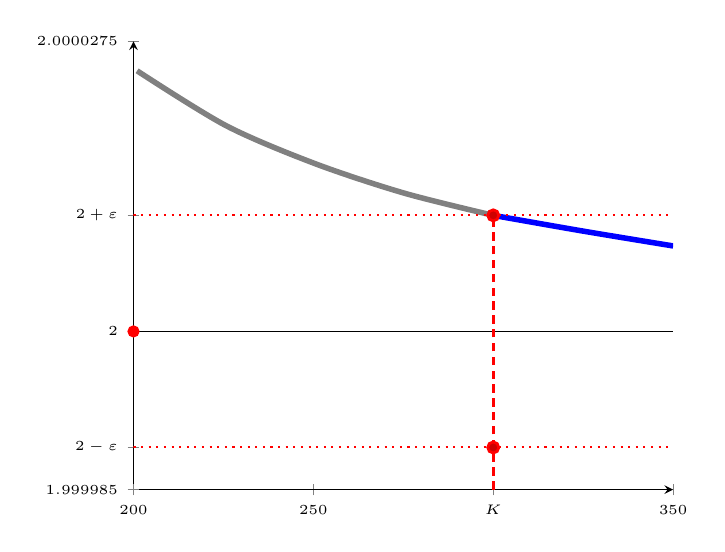
\begin{tikzpicture}[scale=1.0]
          \begin{axis}[axis lines=center,xmin=200,xmax=350,ymin=1.999985,ymax=2.0000275,
          y tick label style={/pgf/number format/.cd,fixed,precision=7,
          set thousands separator={},
          },
          x tick label style={/pgf/number format/.cd,
          scaled x ticks = false,
          set decimal separator={},
          set thousands separator={},
          },
            extra x ticks={200.0},
            extra y ticks={1.999985},
            xtick={200,250,300,350},
            xtick={100,250,300,350},
            xticklabels={200,250,$K$,350},
            ytick={1.999985,1.999989, 2.0,2.000011,2.0000275},
            yticklabels={1.999985,$2 - \varepsilon$,2,$2 + \varepsilon$,2.0000275},
            tick label style={font=\tiny}]
            \addplot[line width=2pt,gray,domain=201:300,samples=5,smooth] {2 + 1/(x^2)};
            \addplot[line width=2pt,blue,domain=300:350,samples=3,smooth] {2 + 1/(x^2)};
            \addplot[only marks,mark=*,red] coordinates { (200,2) };
            \addplot+[xcomb,no marks,thick, line width=0.3pt,black] plot coordinates
	           {(200,2) (350,2)};
            \addplot+[xcomb,no marks,dotted, line width=0.75pt,red] plot coordinates
                {
                    (300,2.000011) (350,2.000011)
                    (300,1.999989) (350,1.999989)
                };
            \addplot+[ycomb, line width=1pt,red] plot coordinates
	           {(300,1.999989) (300,2.000011)};
         \end{axis}
        \end{tikzpicture}
    \end{center}

    \paragraph*{Végtelenben vett végtelen határérték\\}

    \noindent \emph{Mínusz végtelenben vett mínusz végtelen határérték}:
    \begin{center}
        $\lim\limits_{x \to \boldsymbol{-\infty}}f = \boldsymbol{-\infty}$\\
        $\Updownarrow$\\
        $\forall K \in \mathbb{R} \qquad \exists \omega \in \mathbb{R}\ \text{(küszöbszám)} \qquad \forall x \in D_{f}\quad \Big[x \boldsymbol{<} \omega:\ f(x) \boldsymbol{<} K\Big]$
    \end{center}
    \noindent \emph{Mínusz végtelenben vett plusz végtelen határérték}:
    \begin{center}
        $\lim\limits_{x \to \boldsymbol{-\infty}}f = \boldsymbol{+\infty}$\\
        $\Updownarrow$\\
        $\forall K \in \mathbb{R} \qquad \exists \omega \in \mathbb{R}\ \text{(küszöbszám)} \qquad \forall x \in D_{f}\quad \Big[x \boldsymbol{<} \omega:\ f(x) \boldsymbol{>} K\Big]$
    \end{center}

    \noindent \emph{Plusz végtelenben vett mínusz végtelen határérték}:
    \begin{center}
        $\lim\limits_{x \to \boldsymbol{+\infty}}f = \boldsymbol{-\infty}$\\
        $\Updownarrow$\\
        $\forall K \in \mathbb{R} \qquad \exists \omega \in \mathbb{R}\ \text{(küszöbszám)} \qquad \forall x \in D_{f}\quad \Big[x \boldsymbol{>} \omega:\ f(x) \boldsymbol{<} K\Big]$
    \end{center}
    \noindent \emph{Plusz végtelenben vett plusz végtelen határérték}:
    \begin{center}
        $\lim\limits_{x \to \boldsymbol{+\infty}}f = \boldsymbol{+\infty}$\\
        $\Updownarrow$\\
        $\forall K \in \mathbb{R} \qquad \exists \omega \in \mathbb{R}\ \text{(küszöbszám)} \qquad \forall x \in D_{f}\quad \Big[x \boldsymbol{>} \omega:\ f(x) \boldsymbol{>} K\Big]$
    \end{center}

    \subsection*{Határérték és algebrai műveletek}

    Legyen $A,\ B,\ \lambda \in \mathbb{R}$, és $\alpha \in \overline{\mathbb{R}}$. Tegyük fel, hogy
    \[
        \lim_{x \to \alpha} f(x) = A\qquad \Big|\qquad \lim_{x \to \alpha}g(X) = B
    \]
    Ekkor léteznek az alábbi határértékek és fennállnak a következő összefüggések:
    \begin{enumerate}
      \item \emph{Szorzás konstanssal}: $\lim\limits_{x \to \alpha} (\lambda \cdot f) = \left\{ \begin{array}{rl}
                                                                                          \lambda \cdot A &, \text{ha}\ \lambda \neq 0 \\
                                                                                          0 &, \text{ha}\ \lambda = 0
                                                                                        \end{array} \right.
      $
      \item \emph{Összeg, különbség}: $\lim\limits_{x \to \alpha} (f \pm g) = A \pm B$
      \item \emph{Szorzat}: $\lim\limits_{x \to \alpha} (f \cdot g) = A \cdot B$
      \item \emph{Hányados}: $\lim\limits_{x \to \alpha}\ddfrac{f}{g} = \ddfrac{A}{B}$ ($B \neq 0$)
      \item \emph{Hatványozás}: $\lim\limits_{x \to \alpha} (f^{n}) = A^{n},\ n \in \mathbb{Z}$ (feltéve, hogy $A^{n}$ értelmezve van)
    \end{enumerate}
\newpage
    \noindent Az "eldönthetetlen" $0^{0}, 1^{\pm\infty}, (\pm\infty)^{0}, (+\infty) + (-\infty),\ 0 \cdot \pm\infty,\ \ddfrac{0}{0},\ \ddfrac{\pm\infty}{\pm\infty}$ limeszeknél a függvényt próbáljuk meg úgy átalakítani, hogy az új kifejezés limesze már eldönthető legyen.\\

    \noindent Példák:
    \[
        \lim\limits_{x \to \infty}x^{2} - x + 2 = \infty -\infty + 2 = ?,\ de
    \]
    \[
        \lim\limits_{x \to \infty}x^{2} - x + 2 = \lim\limits_{x \to \infty}x^{2}(1 - \ddfrac{1}{x} + \ddfrac{2}{x^{2}}) = \infty \cdot (1 - 0 + 0) = \infty \cdot 1 = \infty
    \]

    \[
        \lim\limits_{x \to \infty}\ddfrac{x^{2} - x + 2}{2x^{2}+3} = \ddfrac{\infty}{\infty} = ?,\ de
    \]
    \[
        \lim\limits_{x \to \infty}\ddfrac{x^{2}(1 - \ddfrac{1}{x} + \ddfrac{2}{x^{2}})}{x^{2}(2+\ddfrac{3}{x^{2}})} = \lim\limits_{x \to \infty}\ddfrac{1 - \ddfrac{1}{x} + \ddfrac{2}{x^{2}}}{2+\ddfrac{3}{x^{2}}} = \lim\limits_{x \to \infty}\ddfrac{\textbf{1} - \underbrace{\ddfrac{1}{x}}_{\rightarrow 0} + \underbrace{\ddfrac{2}{x^{2}}}_{\rightarrow 0}}{\textbf{2}+\underbrace{\ddfrac{3}{x^{2}}}_{\rightarrow 0}} = \ddfrac{\textbf{1}}{\textbf{2}}
    \]

    \subsection*{Féloldali határértékek}

    \noindent Az $f$ függvény \textbf{\emph{jobb oldali határértéke}} az $a$ helyen az $A$ szám (jelölése: $\lim\limits_{x \to a^{+}} = \lim\limits_{x \to a+0} = A$),\ ha
    \[
        \forall \varepsilon > 0\qquad \exists \delta > 0\qquad \forall x\ \Big[\boldsymbol{a < x < a + \delta}\ \Rightarrow \big|f(x) - A\big| < \varepsilon\Big]
    \]

    \noindent Az $f$ függvény \textbf{\emph{bal oldali határértéke}} az $a$ helyen az $A$ szám (jelölése: $\lim\limits_{x \to a^{-}} = \lim\limits_{x \to a-0} = A$),\ ha
    \[
        \forall \varepsilon > 0\qquad \exists \delta > 0\qquad \forall x\ \Big[\boldsymbol{a - \delta < x < a} \Rightarrow \big|f(x) - A\big| < \varepsilon\Big]
    \]

    \noindent \textbf{Tétel}. Az $f$ függvénynek pontosan akkor létezik az $a$ helyen határértéke, ha ugyanitt létezik mind a jobb, mind a bal oldali határértéke és ezek egyenlőek, azaz
    \[
        \lim\limits_{x \to a^{+}}f(x) = \lim\limits_{x \to a^{-}}f(x)
        \Leftrightarrow
        A \lim\limits_{x \to a}f(x)
    \]

	\section*{Függvények folytonossága}

    \noindent A függvény $a$-beli folytonossága azt jelenti, hogy akármilyen kicsi $\varepsilon$ hibakorlátot is szabunk, mindig lesz az $a$ körül olyan kis $( a-\delta, a+\delta )$ intervallum, amelyen belüli $x$-ekre a függvény $f(x)$ értékei a hibakorlátnál ($\varepsilon$-nál) kisebb mértékben térnek el $f(a)$-tól.\\
	
    \noindent \emph{Formálisan}: Az $f : \mathbb{R} \to \mathbb{R}$ függvény az $a \in \mathcal{D}_{f}$ pontban folytonos, ha
    \begin{center}
        $\forall \varepsilon > 0\qquad \exists \delta > 0$\qquad $\forall x \in K_{\delta}(a) : f(x) \in K_{\varepsilon}\Big(f(a)\Big)$ \\
        $\Updownarrow$\\
        $\forall \varepsilon > 0\qquad \exists \delta > 0$\qquad $\forall x \in \mathcal{D}_{f}\quad  \Big[0 < \big|x-a\big| < \delta \Rightarrow \big|f(x)-f(a)\big| < \varepsilon\Big]$\\
    \end{center}

	\noindent A pontbeli folytonosság jelölése: $f \in \mathcal{C}[a]$.

    \subsubsection*{Folytonos függvények és a határérték kapcsolata}

    \noindent Az $f : \mathbb{R} \to \mathbb{R}$ függvény folytonos az $a \in \mathcal{D}_{f} \cap \mathcal{D}'_{f}$ pontban, ha
    \[
        \exists \lim\limits_{x \to a}f(x)\ \text{véges határérték és}\ \lim\limits_{x \to a}f(x) = f(a)
    \]

    \noindent Ha $f$ a $c$ helyen nincs értelmezve, de létezik az $L = \lim\limits_{c}f$ határérték, akkor az
    \[
        F(x) = \left\{\begin{array}{cc}
                        f(x) & , \text{ha}\ x \neq c \\
                        L & , \text{ha}\ x = c
                      \end{array}
         \right.
    \]
    függvényt az $\textbf{f}$ $\emph{\textbf{c}}$-re való \emph{\textbf{kiterjesztésének}} nevezzük.\\

    \noindent Például $\ddfrac{\sin{x}}{x}$ folytonosan kiterjeszthető az egész számegyenesen.
    \[
        F(x) = \left\{\begin{array}{cc}
                        \ddfrac{\sin{x}}{x} & , \text{ha}\ x \neq 0 \\
                        1 & , \text{ha}\ x = 0
                      \end{array}
         \right.
    \]

    \noindent \textbf{Állítás:} Az $f: [a,b] \rightarrow \mathbb{R}$ pontosan akkor folytonos, ha
    \begin{itemize}
        \item $[a, b]$ intervallum minden belső $c$ pontjában $\lim\limits_{x \to c}f = f(c)$
        \item az $a$ végpontban $\lim\limits_{x \to a^{+}}f = f(a)$
        \item a $b$ végpontban $\lim\limits_{x \to b^{-}}f = f(b)$
    \end{itemize}

    \noindent Az $a$ \textbf{megszüntethető szakadási pontja/helye} az $f$ függvénynek, ha
    \[
        \exists \lim\limits_{x \to a}f,\ \text{de}\ \lim\limits_{x \to a}f \neq f(a)
    \]

    \noindent Példa:

    $f(x) = \left\{
      \begin{array}{rc}
        \ddfrac{\sin(x)}{x}, & x \in \mathbb{R}\backslash\{0\} \\
        0, & x = 0
      \end{array}
    \right.$

      \begin{center}
          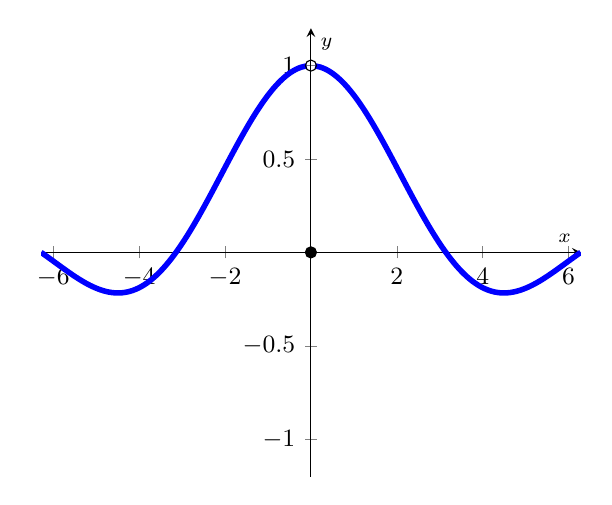
\begin{tikzpicture}[scale=1.0]
              \begin{axis}[axis lines=middle,xmin=-2*pi,xmax=2*pi,ymin=-1.2,ymax=1.2,
                xlabel=$\scriptstyle x$,
                ylabel=$\scriptstyle y$,
                tick label style={font=\small}]
                \addplot[no marks,domain=-2*pi:-0.1,samples=50,smooth,line width=2pt,blue]{sin(deg(x))/x};
                \addplot[no marks,domain=0.1:2*pi,samples=50,smooth,line width=2pt,blue]{sin(deg(x))/x};
                \addplot [only marks,mark=*] coordinates { (0,0) };
                \addplot [only marks,mark=o] coordinates { (0,1) };
              \end{axis}
            \end{tikzpicture}
        \end{center}

        \begin{itemize}
          \item $f \in \mathcal{C}[a],\ \forall a \neq 0$
          \item a = 0,\ \text{megszüntethető szakadási hely, mert}\ $\lim\limits_{x \to 0}\ddfrac{sin(x)}{x} = 1 \neq f(0) = 0$
        \end{itemize}

    \noindent Az $a$ \textbf{ugráshelye} az $f$-nek, ha $\lim\limits_{x \to a^{+}}$ és $\lim\limits_{x \to a^{-}}$ végesek, de $\lim\limits_{x \to a^{+}} \neq \lim\limits_{x \to a^{-}}$.\\

    $f(x) = \left\{
      \begin{array}{rc}
        0, & \text{ha}\ x < 0 \\
        1, & \text{ha}\ x \geq 0
      \end{array}
    \right.$

      \begin{center}
          \begin{tikzpicture}[scale=1.0]
              \begin{axis}[axis lines=middle,xmin=-5.0,xmax=5.0,ymin=-1.0,ymax=2.0,
                xlabel=$\scriptstyle x$,
                ylabel=$\scriptstyle y$,
                tick label style={font=\small}]
                \addplot[no marks,domain=-5.0:-0.1,samples=5,smooth,line width=2pt,blue]{0};
                \addplot [only marks,mark=o] coordinates { (0,0) };
                \addplot [only marks,mark=*] coordinates { (0,1) };
                \addplot[no marks,domain=0.1:5,samples=5,smooth,line width=2pt,blue]{1};
              \end{axis}
            \end{tikzpicture}
        \end{center}

    \noindent Az $a$ \textbf{hézagpontja} az $f$-nek, ha $\lim\limits_{x \to a^{+}} \pm \infty$ és $\lim\limits_{x \to a^{-}} = \pm \infty$, de $f$ nincs értelmezve $a$-ban.\\

    \noindent Példa: $\ddfrac{x^2-1}{x-1}$ hézagpontja (x=1)-ben van.

      \begin{center}
          \begin{tikzpicture}[scale=1.0]
              \begin{axis}[axis lines=middle,xmin=-5.0,xmax=5.0,ymin=-5.0,ymax=5.0,
                xlabel=$\scriptstyle x$,
                ylabel=$\scriptstyle y$,
                xtick={-5,-1,0,1,5},
                ytick={-5,0,1,5},
                tick label style={font=\small}]
                \addplot [only marks,mark=o] coordinates { (1,2) };
                \addplot[no marks,domain=-5.0:0.925,samples=100,smooth,line width=2pt,blue]{(x^2-1)/(x-1)};
                \addplot[no marks,domain=1.075:5.0,samples=100,smooth,line width=2pt,blue]{(x^2-1)/(x-1)};
              \end{axis}
            \end{tikzpicture}
        \end{center}

    \subsubsection*{A műveletek és a folytonosság kapcsolata}

    \noindent Ha $f \in \mathcal{C}[a]$ és $g \in \mathcal{C}[a]$, akkor
    \begin{itemize}
            \item $\lambda f \in \mathcal{C}[a]$ ($\lambda \in \mathbb{R}$)
            \item $f + g \in \mathcal{C}[a], f \cdot g \in \mathcal{C}[a]$.
            \item $\ddfrac{f}{g} \in \mathcal{C}[a]$, feltéve hogy $g(a) \neq 0$.\\
    \end{itemize}

    \noindent \textbf{Tétel}: Ha $g \in \mathcal{C}[a]$ és $f(x) \in \mathcal{C}[g(a)]$, akkor $f \circ g \in \mathcal{C}[a]$, azaz $f\big(g(x)\big) \in \mathcal{C}[a]$.\\

    \noindent \emph{Megjegyzés}: Visszafelé nem feltétlenül igaz az állítás.\\
    Legyen $f : = sgn(x)$ és $g := -sgn(x)$. \\
    Ekkor $f + g$ az azonosan nulla függvény, és $f + g \in \mathcal{C}[0]$, de $f \not \in \mathcal{C}[0]$ és $g \not \in \mathcal{C}[0]$.\\\\

    \noindent Az $f$ függvény folytonos az $I$ intervallumon, ha az intervallumra megszorított $f|_{I}$ függvény folytonos. Azaz, ha
    \[
        \forall \alpha \in I: f \in \mathcal{C}[\alpha]
    \]

    \noindent Példa olyan függvényre, amely folytonos egy zárt intervallumban. A $f(x)=\ddfrac{x+1}{x-1}$ függvény például folytonos az $a=3$ pontban a $[2,4]$ intervallumon.

    \begin{center}
        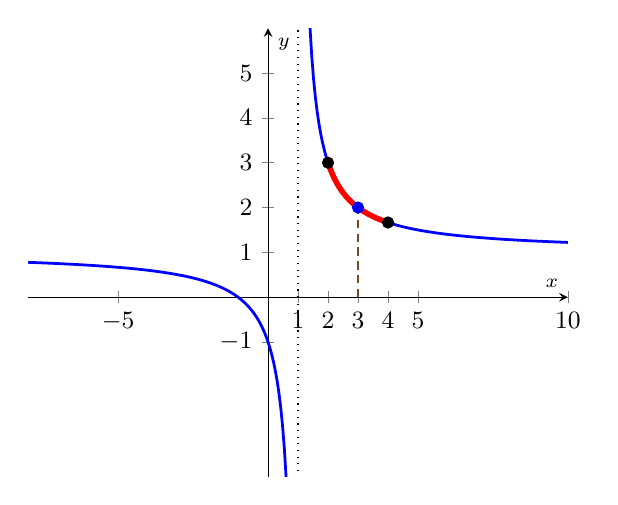
\begin{tikzpicture}[scale=1.0]
          \begin{axis}[axis lines=middle,xmin=-8.0,xmax=10.0,ymin=-4.0,ymax=6.0,
            xlabel=$\scriptstyle x$,
            ylabel=$\scriptstyle y$,
            xtick={-5,0,1,2,3,4,5,10},
            ytick={-1,0,1,2,3,4,5},
            tick label style={font=\small}]
            \addplot[no marks,line width=1pt,blue,domain=-8.0:0.9,samples=150] {(x+1)/(x-1)};
            \addplot[no marks,line width=1pt,blue,domain=1.1:10.0,samples=150] {(x+1)/(x-1)};
            \addplot[no marks,line width=2pt,red,domain=2.0:4.0,samples=150] {(x+1)/(x-1)};
            \addplot [only marks,mark=*] coordinates { (2,3) };
            \addplot [only marks,mark=*] coordinates { (4,5/3) };
            \addplot [only marks,mark=*,blue] coordinates { (3,2) };
            \addplot+[ycomb,no marks] plot coordinates
	           {(3,0) (3,2)};
            \addplot+[ycomb,no marks, dotted] plot coordinates
	           {(1,-4) (1,6)};
          \end{axis}
        \end{tikzpicture}
    \end{center}

    \noindent Az $f$ függvény folytonos, ha értelmezési tartománya minden pontjában folytonos.\\
    \[
        \forall x \in \mathcal{D}_{f} : f \in \mathcal{C}[x],\ \text{akkor}\ f \in \mathcal{C}\ \text{($f$ folytonos függvény)}
    \]

    \noindent Példa olyan függvényre, amely az egész számegyenesen folytonos.\\
    Legyen $f(x) = \ddfrac{1}{x^{2} + 2}$

    \begin{center}
        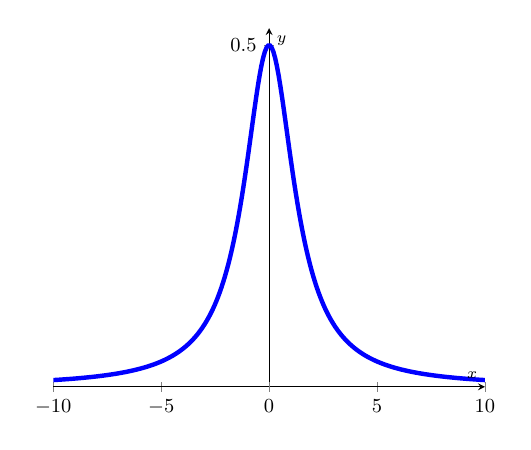
\begin{tikzpicture}[scale=0.8]
          \begin{axis}[axis lines=middle,xmin=-10,xmax=10,ymin=0.0,ymax=0.525,
            xlabel=$\scriptstyle x$,
            ylabel=$\scriptstyle y$,
            xtick={-10,-5,0,5,10},
            ytick={0,0.5},
            extra x ticks={0},
            tick label style={font=\small}]
            \addplot[no marks,line width=2pt,blue,domain=-10.0:10.0,samples=250] {1/((x)^2 + 2)};
          \end{axis}
        \end{tikzpicture}
    \end{center}

    \subsubsection*{Intervallumon folytonos függvények tulajdonságai}

	\textbf{Tétel} \emph{(Bolzano)}. Tegyük fel, hogy valamely $-\infty < a < b < +\infty$ esetén az\\
    $f \in \mathcal{C}[a,b]$ és $f(a) \cdot f(b) < 0$ (ellenkező előjelű), ekkor
    \[
        \exists \xi \in (a,b) : f(\xi) = 0
    \]

    \noindent \textbf{Tétel} \emph{(Bolzano-Darboux)}. Ha $f \in C[a,b]$, és legyen $d$ egy tetszőleges szám a $f(a)$ és $f(b)$ között. Ekkor
    \[
        \exists c \in [a,b] : d = f(c)
    \]

    \noindent Ez előző tétel azt mondja, hogy egy intervallumon folytonos függvény ha felvesz két értéket, akkor e két szám közötti minden értéket felvesz, ami azt jelenti, hogy egy intervallum folytonos képe intervallum.
	
	\subsection*{Weierstrass-tétel}
	
    \noindent Ha $f \in \mathcal{C}[a,b]$, akkor van olyan $\alpha, \beta \in [a,b]$, amelyekre teljesül, hogy $\forall x \in [a,b]$-re
    \[
        f(\alpha) \leq f(x) \leq f(\beta)
    \]

    \noindent Ez a tétel azt mondja, hogy $f_{\big|[a,b]}$ korlátos (hiszen $f(\alpha)$ és $f(\beta)$ között van a függvény minden értéke), sőt van minimuma és van maximuma is az $f_{\big|[a,b]}$ függvénynek. \\

    \noindent A Bolzano- és a Weierstrass-tétel következménye, hogy egy \emph{zárt}, \emph{korlátos} intervallum folytonos képe is \emph{korlátos} és \emph{zárt} intervallum.\\

    \noindent \emph{Tétel}: Ha $f \in \mathcal{C}[a,b]$, akkor $f$ korlátos $[a,b]$-ben.

    \paragraph*{Az inverzfüggvény folytonossága}

    \noindent \textbf{Tétel}: Legyen $I \in \mathbb{R}$ intervallum, és $f : I \to \mathbb{R}$ szigorúan monoton. Tegyül fel, hogy $f \in \mathcal{C}[a]$, ahol $a \in I$. Legyen továbbá $b := f(a)$. Ekkor $f^{-1} \in \mathcal{C}[b]$\\

    \noindent Az $f$ függvény értelmezési tartományának egy $a$ pontjában \textbf{jobbról folytonos}, ha
    \[
        \forall \varepsilon > 0\qquad \exists \delta > 0\qquad \forall x \ \Big[0 \leq x - a < \delta : \big|f(x) - f(a)\big| < \varepsilon\Big]
    \]

    \noindent Az $f$ függvény értelmezési tartományának egy $a$ pontjában \textbf{balról folytonos}, ha
    \[
        \forall \varepsilon > 0\qquad \exists \delta > 0\qquad \forall x \ \Big[0 \leq a - x < \delta : \big|f(x) - f(a)\big| < \varepsilon\Big]
    \]

    \noindent \textbf{Tétel.} (Átviteli elv) Az $f$ függvény akkor és csak akkor folytonos az $a$ pontban, ha értelmezve van az $a$ pont környezetében, és minden $x_{n} \to a$ sorozatra $f(x_{n}) \to f(a)$.\\

    \noindent Példa olyan függvényre, amely mindenütt értelmezett, de sehol sem folytonos

    \[
        D(x)= \left\{ \begin{array}{rl}
                        1 & \text{, ha}\ x \in \mathbb{Q} \\
                        0 & \text{, ha}\ x \not \in \mathbb{Q}
                      \end{array}
         \right.
    \]
    ahol a $D(x)$ függvény a \emph{Dirichlet} függvény. Ha sorozat minden tagja racionális szám, ilyenkor ez a függvény mindig $1$ értéket ad. Mégsem mondhatjuk, hogy a függvény értékeinek a sorozata tart az egyhez, hiszen bármelyik két racionális szám között végtelen sok irracionális szám van.\\

    \noindent Az $a$ \textbf{szakadási pontja/helye} az $f$ függvénynek, ha $f$ az $a$ pontban nem folytonos ($f \not \in \mathcal{C}[a]$).\\

    \noindent \textbf{Példa} olyan függvény, amely egy korlátos, zárt intervallumban végtelen sok helyen szakad.
    Legyen
    \[
        f:[0,1] \rightarrow \mathbb{R} = \left\{ \begin{array}{cc}
                                           \ddfrac{1}{\Big\lceil\frac{1}{x}\Big\rceil} & ,\ \text{ha}\ x \neq 0 \\
                                           0 & ,\ \text{ha}\ x = 0
                                         \end{array} \right.
        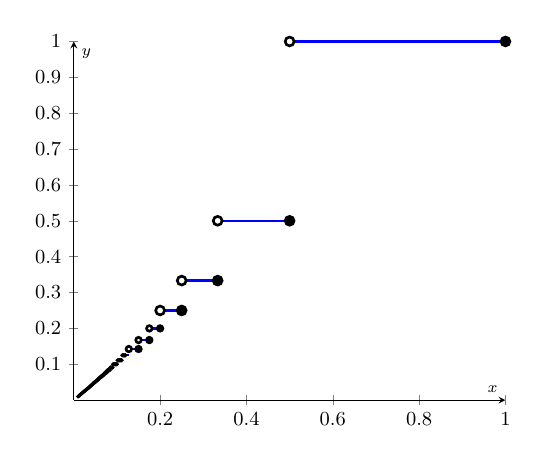
\begin{tikzpicture}[scale=0.8]
          \begin{axis}[axis lines=middle,xmin=0.0,xmax=1.0,ymin=0.0,ymax=1.0,
            clip=false,
            every axis plot/.style={very thick},
            xlabel=$\scriptstyle x$,
            ylabel=$\scriptstyle y$,
            ytick={0,0.1,0.2,0.3,0.4,0.5,0.6,0.7,0.8,0.9,1.0},
                tick label style={font=\small}]
            \addplot+[jump mark left,mark=none,line width=1.0pt,blue,domain=0.12:1.0,samples=120] {1/(floor(1/x))};
            \addplot[only marks,mark=*, mark size=2pt]coordinates{(0.5,0.5) (1.0,1.0) (0.33333, 0.33333) (0.25, 0.25)};
            \addplot[only marks,fill=white, mark size=2pt]coordinates{(0.5,1.0) (0.33333, 0.5) (0.25, 0.33333) (0.2, 0.25)};

            \addplot[only marks,mark=*, mark size=1.25pt]coordinates{(0.2,0.2) (0.175,0.1675) (0.15, 0.1425)};
            \addplot[only marks,fill=white, mark size=1.25pt]coordinates{(0.175,0.2) (0.15, 0.1675) (0.1275, 0.1425)};

            \addplot+[only marks,mark=*, mark size=0.25pt,line width=1.0pt,black,domain=0.01:0.12,samples=100,fill=blue] {1/(floor(1/x))};
          \end{axis}
        \end{tikzpicture}
    \]


    \noindent \emph{Állítás:} Ha $\exists \lim\limits_{x \to a^{+}}$ f, és $\lim\limits_{x \to a^{+}} = f(a)$, akkor $f$ \textbf{jobbról folytonos} az $a$-ban.\\

    \noindent \emph{Állítás:} Ha $\exists \lim\limits_{x \to a^{-}}$ f, és $\lim\limits_{x \to a^{-}} = f(a)$, akkor $f$ \textbf{balról folytonos} az $a$-ban.\\

    \subsection*{Egyenletes folytonosság}

    \noindent Ha $H \subset \mathbb{R}$ kompakt és $f: H \to \mathbb{R}$ folytonos függvény, akkor $R_{f}$ (a fv. értékkészlete) is kompakt.\\

    \noindent Akkor mondjuk, hogy az $f : \mathbb{R} \to \mathbb{R}$ függvény a $H \subset D_{f}$ halmazon \emph{egyenletesen folytonos}, ha
    \[
        \forall \varepsilon > 0\qquad \exists \delta > 0\qquad \forall x,\ y \in H\ \Big[0 < \big|x-y\big| < \delta : \big|f(x)-f(y)\big| < \varepsilon\Big]
    \]

	\subsubsection*{Heine-tétel}
	
    Ha $H \subset \mathbb{R}$ kompakt halmaz és $\big(f: H \to \mathbb{R}\big) \in \mathcal{C}$, akkor az $f$ a $H$ halmazon egyenletesen folytonos.

%    \subsection*{Sorozatok}

%	Az $f$ függvényt \textbf{sorozat}nak nevezzük, ha $\mathcal{D}_{f} = \mathbb{N}$. Jelölése: $\big(a_{n}\big)$ vagy $\big\{a_{n}\big\}$.\\

%    \noindent Az $\big(a_{n}\big)$ sorozattal az $n \in N$ számhoz rendelt értéket a sorozat $\textbf{n}$-\textbf{edik tag}jának nevezzük.
%    \begin{itemize}
%        \item \text{Jelölése}: $a_{n}$
%    \end{itemize}

%    \noindent Ha egy $\big(a_{n}\big)$ sorozat értékkészlete
%    \begin{itemize}
%      \item $R_{f} = \mathbb{R}$ \emph{valós számsorozat}nak,
%      \item $R_{f} = \mathbb{C}$ \emph{komplex számsorozat}nak,
%      \item $R_{f} \subset \mathbb{R}^{n}$ (n-dimenziós euklideszi tér) $R^{n}$-beli \emph{vektorsorozat}nak nevezzzük.
%    \end{itemize}

%	\paragraph*{Konvergens}
	
%	Egy $x = (a_{n}) : \mathbb{N} \to \mathbb{R}$ számsorozat konvergens, ha
%    \[
%        \exists A \in \mathbb{R},\ \forall \varepsilon > 0,\ \exists k \in \mathbb{N},\ \forall n \in \mathbb{N},\ n > k : \Big|a_{n} - A\Big| < \varepsilon.
%    \]
%	\noindent Tehát bármilyen kicsi $\varepsilon$ esetén egy sorszám után $k$ a sorozat összes tagja $\varepsilon$ távolságnál közelebb van $A$-hoz.\\

%    \noindent Ha az $\big(a_{n}\big):\ \mathbb{N} \to \mathbb{R}$ sorozat konvergens, akkor egyetlen olyan $A \in \mathbb{R}$ szám létezik, amelyre a konvergencia (előző def.) teljesül.\\
%    Ezt az $A$ számot az $\big(a_{n}\big)$ \textbf{sorozat határértékének} nevezzük:
%    \[
%        lim (a_{n}) := A\qquad (n \to \infty)
%    \]

%    \noindent Ha az $\big(a_{n}\big)$ sorozat nem konvergens, akkor \textbf{divergens}nek nevezzük.\\

%    \noindent Akkor mondjuk, hogy az $a =\big(a_{n}\big)$ valós vagy komplex számsorozat felülről korlátos, ha létezik olyan $K$ szám, hogy minden $n \in \mathbb{N}$ indexre fennáll az $\big|a_{n}\big| \leq K$ egyenlőtlenség, azaz:
%    \[
%        \exists K \in \mathbb{R},\ \text{hogy}\ \forall n \in \mathbb{N}: a_{n} \leq K.
%    \]
%    A $K$ számot a sorozat \textbf{felső korlát}jának nevezzük.\\

%    \noindent Akkor mondjuk, hogy az $a =\big(a_{n}\big)$ valós vagy komplex számsorozat \textbf{alulról korlátos}, ha létezik olyan $k$ szám, hogy minden $n \in \mathbb{N}$ indexre fennáll  az $\big|a_{n}\big| \geq k$ egyenlőtlenség, azaz:
%    \[
%        \exists k \in \mathbb{R},\ \text{hogy}\ \forall n \in \mathbb{N}: a_{n} \geq k.
%    \]
%    A $k$ számot a sorozat \textbf{alsó korlát}jának nevezzük.\\

%	\noindent Az $A \subset \mathbb{R}$ \textbf{zárt}, ha bármely $(a_{n}): \mathbb{N} \to A$ sorozatnak van olyan $\big(a_{\nu_{n}}\big)$ részsorozata, amely konvergens és $\lim{(a_{\nu_{n}})} \in A$.\\

    \section*{Hatványsorok}

%	\paragraph*{Függvénysorozat, függvénysor}
	
%    Az olyan sorozatot, amelynek értékei azonos értelmezési tartománnyal rendelkező függvények, \textbf{függvénysorozat}nak nevezzük.\\

%    \noindent Az $f_n:D \to \mathbb{R},\ n \in \mathbb{N}$ függvényeknek a közös értélmezési tartománya $D \neq \emptyset$.\\
%    Ezen függvények végtelen összegét nevezzük függvénysornak:
%    \[
%        \sum\limits_{n=1}^{\infty}f_n=f_1+f_2+ \ldots+f_n+\ldots = \Big(f_{n}(x)\Big)
%    \]

%    \noindent Az $f_1,f_2,f_3,...,f_n,...$ függvények a függvénysor tagjai. Az $\Big(f_{n}(x)\Big)$ sorozat $n$-edik tagja $f_{n}(x)$.\\

%    \noindent \emph{Megjegyzés}. Az $x$ az adott $f_{n}$ függvény értelmezési tartományából származó valós szám.\\

%    \noindent \textbf{Definíció}. Egy $\Big(f_{n}(x)\Big)$ függvénysorozatra azt mondjuk, hogy konvergens és tart egy $f(x)$ függvényhez, ha bármely $x$ esetén, amikor tetszőleges pozitív $\varepsilon$ valós számhoz létezik olyan $N_{\varepsilon} \in %\mathbb{Z}^{+}$  küszöbindex, hogy ha $n \in N_{\varepsilon}$, akkor $\Big|f_{n}(x) - f(x)\Big| < \varepsilon$. Az $f(x)$ függvényt \textbf{határfüggvénynek} nevezzük.\\

%    \noindent \emph{Megjegyzés}. A megfelelő $N_{\varepsilon}$ értéke általában az $\varepsilon$-on kívül az adott $x$ értékétől is függ, mivel a konvergencia sebessége általában minden $x$ esetén más és más.\\

    \noindent Legyen $x,\ x_{0} \in \mathbb{R}$ és $a =(a_{0}, a_{1},\ldots, a_{n}, \ldots)\quad (a_{n} \in \mathbb{R})_{n \in \mathbb{N}_{0}}$ egy tetszőleges sorozat. \\
    A következő alakú végtelen sort \textbf{hatványsornak} nevezzük.
    \[
        a_{0} + a_{1}(x-x_{0}) + a_{2}(x-x_{0})^{2}+ \ldots + a_{n}(x-x_{0})^{n} + \ldots = \sum\limits_{n=0}^{\infty}a_{n}(x-x_{0})^{n}
    \]

    \begin{itemize}
        \item $\boldsymbol{a_{i}}\ (i = 0,1,2\ldots)$ számok a \textbf{hatványsor együtthatói}.
        \item $\boldsymbol{x_{0}}$ szám a hatványsor \textbf{középpontja} (centruma).
        \item $\textbf{\emph{x}}$ a hatványsor \textbf{változója}.
    \end{itemize}

%    \noindent Egy $\sum\limits_{n=0}^{\infty}a_{n}(x-x_{0})^{n}$ hatványsorra azt mondjuk, hogy
%    \begin{itemize}
%        \item \emph{konvergens}, ha $\Big|\sum\limits_{n=0}^{\infty}a_{n}(x-x_{0})^{n}\Big| < \infty$ valamely $x$ számokra.
%        \item \emph{divergens}, ha $\Big|\sum\limits_{n=0}^{\infty}a_{n}(x-x_{0})^{n}\Big| = \infty$ valamely $x$ számokra.
%        \item \emph{abszolút konvergens}, ha $\Big|\sum\limits_{n=0}^{\infty}|a_{n}(x-x_{0})^{n}|\Big| < \infty$ valamely $x$ számokra.\\
%    \end{itemize}

    \noindent A $\sum\limits_{n=0}^{\infty}a_{n}(x-x_{0})^{n}$ hatványsor
    \begin{itemize}
        \item konverges, ha $\left|\sum\limits_{n=0}^{\infty}a_{n}(x-x_{0})^{n}\right| < \infty$ valamely x értékekre
        \item divergens, ha $\left|\sum\limits_{n=0}^{\infty}a_{n}(x-x_{0})^{n}\right| = \infty$ valamely x értékekre
        \item abszolút konvergens, ha $\left|\sum\limits_{n=0}^{\infty}\big|a_{n}(x-x_{0})^{n}\big|\right| < \infty$ valamely x értékekre
    \end{itemize}

    \noindent Egy hatványsor \textbf{konvergenciatartománya} alatt azt az $I \in \mathbb{R}$ intervallumot értjük, ahol $\sum\limits_{n=0}^{\infty}a_{n}(x-x_{0})^{n}$ hatványsor konvergens minden $x \in I$ esetén.\\

    \noindent \emph{Megjegyzés}: Az $I$ intervallum mindig egy az $x_{0}$  középpontra szimmetrikus tartomány, azaz $I = \Big(x_{0} - r,\ x_{0} + r\Big)$. Ezt az $r \in \mathbb{R}$ számot \textbf{konvergenciasugárnak} nevezzük.

    \[
        K_{r}(x_{0}) := \Big\{x \in \mathbb{R}\ \Big|\ \big|x-x_{0}\big| < r\Big\}
    \]

    \noindent Az $r$ konvergenciasugarat  a hányadoskritérium segítségével is megtalálhatjuk.\\
    Ez esetben a konvergenciasugár a következőképp számolható ki:
    \[
        r = \lim\limits_{n \to \infty}^{}\Big|\ddfrac{a_{n}}{a_{n+1}}\Big| \qquad (\text{ha létezik})
    \]

    \noindent Példa: $\sum\limits_{n=0}^{\infty}3^{n} \cdot x^{n}$ konvergenciasugara.\\

    \[
        \lim\limits_{}^{}\Big|\ddfrac{a_{n}}{a_{n+1}}\Big| = \ddfrac{3^{n}}{3^{n+1}} = \ddfrac{3^{n}}{3 \cdot 3^{n}} = \ddfrac{1}{3} = r
    \]

    \noindent Mivel $x^n = (x - 0)^{n}$ szerepel, ezért a hatványsor középpontja 0.\\

    \noindent Meg kell vizsgálni a konvergenciát a végpontokban is.\\

    \noindent \textbf{Tétel} (Cauchy-Hadamard): Tekintsük az $r := \ddfrac{1}{\lim\limits_{n \to \infty}^{}\sqrt[n]{|a_{n}|}}$ értéket.\\

    \noindent Amennyiben
    \begin{enumerate}
        \item $|x - x_{0}| < r \quad \sum\limits_{n=0}^{\infty}a_{n}(x-x_{0})^{n}$ \emph{abszolút konvergens}.
        \item $|x - x_{0}| > r \quad \sum\limits_{n=0}^{\infty}a_{n}(x-x_{0})^{n}$ hatványsor \emph{divergens}.
        \item $|x - x_{0}| = r \quad$ (nem mondható semmi a konvergenciáról)
    \end{enumerate}

    \noindent A konvergenciaintervallum végpontjaiban, vagyis $x=r$ és $x=- r$ helyeken külön meg kell vizsgálni, hogy a hatványsor konvergens-e vagy sem.\\

    \noindent \textbf{Tétel}. A hatványsor összegfüggvénye $f(x) = \sum\limits_{n=0}^{\infty}a_{n}(x-x_{0})^{n}$ folytonos. \\

    \noindent \textbf{Tétel}. Ha a $\sum\limits_{n=0}^{\infty}a_{n}(x - x_{0})^{n}$ hatványsor konvergenciasugara $r > 0$, és összeg-függvénye $f(x)$, akkor minden $x \in (- r,r)$-re fennáll, hogy $f(x)$ tetszőlegesen sokszor differenciálható és a deriváltak a következők:
    \[
        f'(x) =\sum\limits_{\boldsymbol{n=1}}^{\infty} a_{n}n(x - x_0)^{n-1} = \sum\limits_{\boldsymbol{n=0}}^{\infty}\boldsymbol{(n+1)} \cdot a_{n+1}(x-x_{0})^{n}
    \]
    \[
        \vdots
    \]
    \[
        f^{(k)}(x) = \sum\limits_{n=0}^{\infty}\boldsymbol{(n+k)} \cdot \boldsymbol{(n+k-1)} \cdot \ldots \cdot \boldsymbol{(n+1)} a_{n+k}(x-x_{0})^{n} = \sum\limits_{n=0}^{\infty} \ddfrac{(n+k)!}{n!} a_{n+k}(x-x_{0})^{n}
    \]
	
%    \noindent \textbf{Tétel} (Abel-tétele): Tekintsük a ${\tiny \sum\limits_{n=0}^{\infty}a_{n}(x-x_{0})^{n}}$ hatványsort, melynek konvergencia sugara $0 < r < \infty$. Amennyiben a hatványsor valamely végpontjában konvergens, azaz
%    \[
%        \Big|\sum\limits_{n=0}^{\infty}(-r-x_{0})^{n}\Big| < \infty\quad \text{vagy}\quad \Big|\sum\limits_{n=0}^{\infty}(r-x_{0})^{n}\Big| < \infty\
%    \]
%    akkor az $f(x) = \sum\limits_{n=0}^{\infty}a_{n}(x-x_{0})^{n}$ összefüggvény folytonosan kiterjed az adott végpontra is, formálisan:
%    \[
%        \lim\limits_{x \to (-r-x_{0})+}^{}f(x) = \sum\limits_{n=0}^{\infty}(-r-x_{0})^{n}\quad \text{illetve}\quad \lim\limits_{x \to (r-x_{0})-}^{}f(x) = \sum\limits_{n=0}^{\infty}(r-x_{0})^{n}
%    \]

    \subsection*{Analitikus függvények}
	
    \noindent Az $f$ függvény az $x_{0}$ pontban \emph{analitikus}, ha $x_{0}$ egy környezetében konvergens hatványsor összegeként áll elő, azaz $\exists r > 0$, hogy
    \[
        f(x) = \sum\limits_{n=0}^{\infty}a_{n}(x-x_{0}),\qquad \big(x \in K_{r}(x_{0})\big)
    \]

    \noindent Az $f$ függvény egy $I$ intervallumon \emph{analitikus}, ha az intervallum minden pontjában az.\\


    \noindent \textbf{Tétel} (Hatványsor egyértelműsége): Ha $f$ \emph{analitikus} $x_{0}$-ban, azaz $\exists r > 0$, hogy $\forall x \in K_{r}(x_{0})$ esetén
    \[
        f(x) = \sum\limits_{n=0}^{\infty}a_{n}(x-x_{0}),\ \text{akkor}\ a_{n} = \ddfrac{f^{(n)}(x_{0})}{n!}
    \]

    \noindent Ez egyben azt is jelenti, hogy $x_{0}$-ban analitikus függvény egyértelműen fejthető $x_{0}$ középpontú hatványsorba, mégpedig
    \[
        f(x) = \sum\limits_{n=0}^{\infty}\ddfrac{f^{(n)}(x_{0})}{n!}(x - x _{0})^{n},\quad x \in K_{r}(x_{0})
    \]

    \noindent \textbf{Következmény}. Minden hatványsor az összegfüggvényének Taylor sora.

    \subsection*{Taylor-polinomok, Taylor-sorok\\}

    \noindent Legyen az $f$ függvény értelmezési tartománya egy $I \subseteq \mathbb{R}$ intervallum és $x_{0}$ az $I$ belső pontja.\\
    Valamint legyen $t_{n}(x)$ olyan $n$-ed fokú polinom, hogy $t^{(k)}(x_{0}) = f^{(k)}(x_{0})$, ahol $k = 0, 1, 2, \ldots, n$.\\

    \noindent Ekkor az $f(x)$ függvény $x_{0}$ központú
    \begin{itemize}
        \item  \textbf{Taylor-sora}:
        \[
            T_{x_0}(f,x) := \sum\limits_{k=0}^{\infty}\underbrace{\ddfrac{f^{(k)}(x_{0})}{k!}}_{a_n} \cdot (x - x_{0})^{k},
        \]
        ahol az $f \in D^{\infty}[x_0]$.\\ \\
        Az $x_{0} = 0$ középpontú speciális Taylor-sort \emph{Maclaurin}-sornak nevezzük. Jelölése: $M(x)$.
        \item \textbf{$\textbf{n}$-ed fokú Taylor-polinomja}:
        \[
            T_{x_0,n}(f,x) := t_{n}(x) = \sum\limits_{k=0}^{n}\ddfrac{f^{(k)}(x_{0})}{k!} \cdot (x - x_{0})^{k},
        \]
        ahol az $f \in D^{(n)}[x_0]$.
    \end{itemize}

    \subsubsection*{Maradéktagok\\}

    A függvény és az azt approximáló $n$-ed fokú Taylor-polinom különbségét megadó függvényt \textbf{maradéktagnak} nevezzük.
    \[
        f(x) - t_{n}(x) = r_{n}(x)
    \]

    \noindent \emph{Megjegyzés}: A Taylor-sor és a függvény eltérése épp az $r_{n}$ függvénysorozat határfüggvénye.\\

    \noindent \textbf{Lagrange-féle maradéktag}: $\xi = x_0 + \alpha(x-x_0) \quad 0 < \alpha < 1$
    \[
        r_{n}^{(L)} = \ddfrac{f^{(n+1)}(\xi)}{(n+1)!}(x-x_{0})^{n+1}
    \]
\newpage

    \noindent A Lagrange-féle maradéktag alapján az approximációs hibára a következő korlát adódik:\\
    
    \noindent Az $f^{(n+1)}(\xi)$ felülről becsülhető az (n+1)-edik derivált abszolútértékének maximumával.\\
    Ez az érték legyen \textbf{M}.\\
    
    \noindent Az $\ddfrac{(x-x_{0})^{n+1}}{(n+1)!}$ pedig majorálható a $\ddfrac{|x-x_{0}|^{n+1}}{(n+1)!}$-sal.\\
    
    \noindent Tehát az $n$-ed fokú Taylor-polinom maximális eltérése az $f$ függvénytől az $x$ helyen:
    \[
        \Big|r_{n}\Big| = \Big|f(x)-t_{n}(x)\Big| \leq M \cdot \ddfrac{(x-x_{0})^{n+1}}{(n+1)!}
    \]

    \noindent \textbf{Következmény}. Ha $\lim\limits_{n \to \infty}r_{n} = 0$, akkor a $t_{n}(x)$ függvény konvergens, és $t_{n}(x) \to f(x)$, így a Taylor-sor előállítja az $f(x)$ függvényt.

	\subsection*{Néhány ismert függvény Taylor-sora, azaz hatványsora\\}
	
    \noindent Ha egy függvény előáll egy hatványsor összegeként, akkor az csak a függvény Taylor-sora lehet, mert ha egy $f(x)$ függvény hatványsorba fejthető, akkor abból az következik, hogy akárhányszor differenciálható.\\
    Továbbá a hatványsor $n$-edik együtthatója $a_n$ a következő alakban áll elő: 
    \[
        a_{n} = \ddfrac{f^{(n)}(x_{0})}{n!}
    \]
    Ez pedig a Taylor-sor definíciója szerint azt jelenti, hogy az $f(x)$ függvényt előállító hatványsor nem más, mint az $f(x)$ Taylor-sora.\\

	\begin{figure}[H]
		\centering
		\includegraphics[width=0.48\linewidth]{img/taylor_sinx_1_3_5_7.png}
		\includegraphics[width=0.48\linewidth]{img/taylor_sinx_51_57.png}
		\caption{Példa 1., 3., 5. és 7. és az 51. és 57. Taylor polinom.}
		\label{fig:newton_pelda}
	\end{figure}

\newpage
    \noindent \textbf{${e^{x}}$ hatványsora és konvergencia tartománya}\\

    \noindent Írjuk fel a $e^{x}$ deriváltjait:
    \[
        (e^{x})' = (e^{x})'' = \ldots = (e^{x})^{(n)} = e^{x}
    \]

    \noindent Ezeket behelyettesítve az $M(x) = \sum\limits_{n=0}^{\infty}\ddfrac{f^{(n)}(0)}{n!} \cdot x^{n}$ képletbe
    \[
        M(x) = 1 + x + \ddfrac{x^2}{2} + \ldots = \sum\limits_{n=0}^{\infty}\ddfrac{x^{n}}{n!}
    \]

    \noindent Ezután azt kell megvizsgálni, hogy az így kapott sor konvergál-e az adott függvényhez. A Lagrange-féle maradéktag szerint az $e^{x}$ függvény és a most kapott hatványsor eltérése egy rögzített $x$ helyen:
    \[
        r_{n}(x) \leq e^{x} \cdot \ddfrac{x^{n+1}}{(n+1)!}
    \]

    \noindent A rögzített $x$ miatt $e^{x}$ egy véges szám, az $\ddfrac{x^{n+1}}{(n+1)!}$ pedig tart 0-hoz, amíg $n$ tart végtelenhez. Ez bármely $x$ valós szám esetén teljesül, tehát a hatványsor az egész számegyenesen konvergál az $e^{x}$ függvényhez.\\

      \begin{center}
          \begin{tikzpicture}[scale=1.0]
              \begin{axis}[axis lines=middle,xmin=-5.0,xmax=5.0,ymin=0.0,ymax=5.0,
                xlabel=$\scriptstyle x$,
                ylabel=$\scriptstyle y$,
                xtick={-5,0,5,8},
                ytick={0,1,5},
                extra x ticks={0},
                tick label style={font=\small}]
                \addplot[no marks,domain=-4.96:4.95,samples=50,smooth,line width=2pt,blue] {exp(x)};
              \end{axis}
            \end{tikzpicture}
        \end{center}
\newpage
    \noindent \textbf{$\sin(x)$ hatványsora és konvergencia tartománya}\\

    \noindent Írjuk fel a $\sin x$ deriváltjait:

    \begin{center}
        $(\sin x)' = \cos x$\\
        $(\sin x)'' = -\sin x$\\
        $(\sin x)''' = -\cos x$\\
        $(\sin x)^{(4)} = \sin x$\\
        $\cdots$
    \end{center}

    \noindent Ezeket behelyettesítve az $M(x) = \sum\limits_{n=0}^{\infty}\ddfrac{f^{(n)}(0)}{n!} \cdot x^{n}$ képletbe
    \begin{spacing}{2}
        \begin{center}
            $M(x) = $\\
            $\ddfrac{f(0)}{0!} + \ddfrac{f'(0)}{1!} + \ddfrac{f''(0)}{2!} + \ddfrac{f'''(0)}{3!} + \ddfrac{f^{(4)}(0)}{4!} + \ddfrac{f^{(5)}(0)}{5!} + \ldots =$\\
            $\ddfrac{\sin(0)}{0!} + \ddfrac{\cos(0)}{1!} + \ddfrac{-\sin(0)}{2!} + \ddfrac{-\cos(0)}{3!} + \ddfrac{\sin(0)}{4!} + \ddfrac{\cos(0)}{5!} + \ldots =$\\
            $\ddfrac{0}{0!} + \ddfrac{1}{1!}x + \ddfrac{0}{2!}x^{2} + \ddfrac{-1}{3!}x^{3} + \ddfrac{0}{4!}x^{4} + \ddfrac{1}{5!}x^{5} + \ldots =$ \\
            $x - \ddfrac{x^3}{3!} + \ddfrac{x^5}{5!} - \ddfrac{x^7}{7!} + \ddfrac{x^9}{9!} - \ldots = \sum\limits_{n=0}^{\infty}(-1)^{n}\ddfrac{x^{2n + 1}}{(2n + 1)!}$
        \end{center}
    \end{spacing}

    \noindent A Lagrange-féle maradéktagból az approximációs hiba egy rögzített $x$ esetén:
    \[
        r_{2n+1}(x) \leq M \cdot \ddfrac{x^{2n+1}}{(2n+1)!}
    \]

    \noindent $M = max\Big\{\big|(sin x)^{(2n+1)}\big|\Big\} = 1$. Így $r_{n} \to 0$, ha $n \to \infty$.\\

    \noindent Tehát a $\boldsymbol{\sin(x) = \sum\limits_{n=0}^{\infty}(-1)^{n}\ddfrac{x^{2n+1}}{(2n+1)!}}$ bármely $x \in \mathbb{R}$ esetén.\\

      \begin{center}
          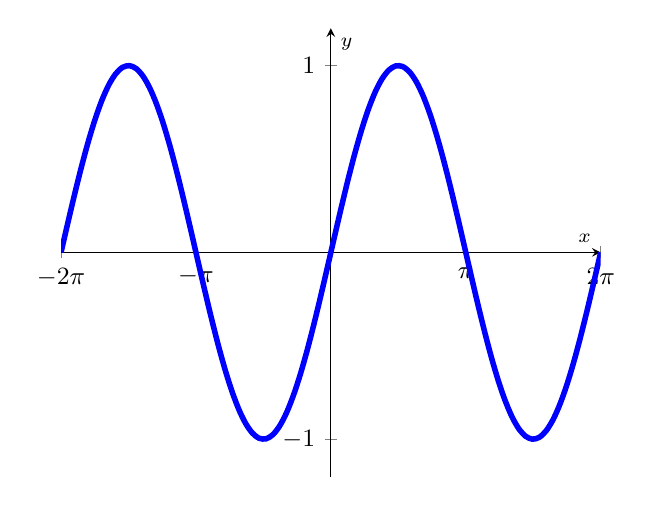
\begin{tikzpicture}[scale=1.0]
              \begin{axis}[axis lines=middle,xmin=-2*pi,xmax=2*pi,ymin=-1.2,ymax=1.2,
                xlabel=$\scriptstyle x$,
                ylabel=$\scriptstyle y$,
                xtick={-2*pi,-pi,0,pi,2*pi},
                xticklabels={$-2\pi$,$-\pi$,0,$\pi$,$2\pi$},
                ytick={-1,0,1},
                tick label style={font=\small}]
                \addplot[no marks,domain=-2*pi:2*pi,samples=80,smooth,line width=2pt,blue]{sin(deg(x))};
              \end{axis}
            \end{tikzpicture}
        \end{center}
\newpage
    \noindent \textbf{$\cos(x)$ hatványsora és konvergencia tartománya}\\

    \noindent Írjuk fel a $\cos x$ deriváltjait:

    \begin{center}
        $(\cos x)' = -\sin x$\\
        $(\cos x)'' = -\cos x$\\
        $(\cos x)''' = \sin x$\\
        $(\cos x)^{(4)} = \cos x$\\
        $\cdots$
    \end{center}

    \noindent Ezeket behelyettesítve az $M(x) = \sum\limits_{n=0}^{\infty}\ddfrac{f^{(n)}(0)}{n!} \cdot x^{n}$ képletbe
    \begin{spacing}{2}
        \begin{center}
            $M(x) = $\\
            $\ddfrac{f(0)}{0!} + \ddfrac{f'(0)}{1!} + \ddfrac{f''(0)}{2!} + \ddfrac{f'''(0)}{3!} + \ddfrac{f^{(4)}(0)}{4!} + \ddfrac{f^{(5)}(0)}{5!} + \ldots =$\\
            $\ddfrac{\cos(0)}{0!} + \ddfrac{-\sin(0)}{1!} + \ddfrac{-\cos(0)}{2!} + \ddfrac{\sin(0)}{3!} + \ddfrac{\cos(0)}{4!} + \ddfrac{-\sin(0)}{5!} + \ldots =$\\
            $\ddfrac{1}{0!} + \ddfrac{0}{1!}x + \ddfrac{-1}{2!}x^{2} + \ddfrac{0}{3!}x^{3} + \ddfrac{1}{4!}x^{4} + \ddfrac{0}{5!}x^{5} + \ddfrac{-1}{6!}x^{6} + \ldots =$ \\
            $1 - \ddfrac{x^2}{2!} + \ddfrac{x^4}{4!} - \ddfrac{x^6}{6!} + \ldots = \sum\limits_{n=0}^{\infty}(-1)^{n}\ddfrac{x^{2n}}{(2n)!}$
        \end{center}
    \end{spacing}

    \noindent A Lagrange-féle maradéktagból az approximációs hiba egy rögzített $x$ esetén:
    \[
        r_{2n}(x) \leq M \cdot \ddfrac{x^{2n}}{(2n)!}
    \]

    \noindent $M = max\Big\{\big|(cos x)^{(2n)}\big|\Big\} = 1$. Így $r_{n} \to 0$, ha $n \to \infty$.\\

    \noindent Tehát a $\boldsymbol{\cos(x) = \sum\limits_{n=0}^{\infty}(-1)^{n}\ddfrac{x^{2n}}{(2n)!}}$ bármely $x \in \mathbb{R}$ esetén.\\

    \noindent Más megközelítésben: $\cos x = (\sin x)'$. Így a $\cos x$ hatványsorához deriváljuk a $\sin x$ hatványsorát.

    \begin{spacing}{2}
        \begin{center}
            $M(x) = \Big(\sum\limits_{n=0}^{\infty}(-1)^{n}\ddfrac{x^{2n+1}}{(2n+1)!}\Big)' = \sum\limits_{n=0}^{\infty}\Big((-1)^{n}\ddfrac{x^{2n+1}}{(2n+1)!}\Big)' = $\\
            $\sum\limits_{n=0}^{\infty}\Big((-1)^{n}\ddfrac{(2n+1)x^{2n}}{(2n+1)(2n)!}\Big) = \sum\limits_{n=0}^{\infty}(-1)^{n}\ddfrac{x^{2n}}{(2n)!}$
        \end{center}
    \end{spacing}

      \begin{center}
          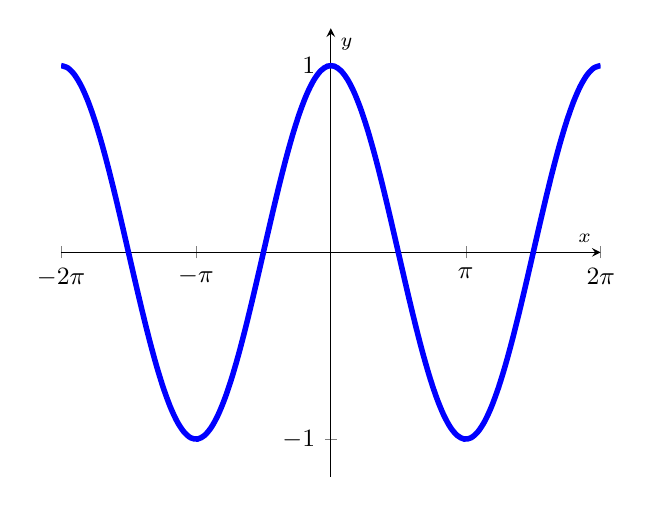
\begin{tikzpicture}[scale=1.0]
              \begin{axis}[axis lines=middle,xmin=-2*pi,xmax=2*pi,ymin=-1.2,ymax=1.2,
                xlabel=$\scriptstyle x$,
                ylabel=$\scriptstyle y$,
                xtick={-2*pi,-pi,0,pi,2*pi},
                xticklabels={$-2\pi$,$-\pi$,0,$\pi$,$2\pi$},
                ytick={-1,0,1},
                tick label style={font=\small}]
                \addplot[no marks,domain=-2*pi:2*pi,samples=80,smooth,line width=2pt,blue]{cos(deg(x))};
              \end{axis}
            \end{tikzpicture}
        \end{center}
\newpage
    \noindent \textbf{$\sinh(x)\ (sh(x))$ hatványsora és konvergencia tartománya}\\

    \noindent Írjuk fel a $\sinh x$ deriváltjait:

    \begin{itemize}
        \item $(\sinh x)^{(n)} = \cosh x$, ha $n$ páratlan, tehát $(\sinh 0)^{(2n+1)} = 1$
        \item $(\sinh x)^{(n)} = \sinh x$, ha $n$ páros, tehát $(\sinh 0)^{(2n)} = 0$
    \end{itemize}

    \noindent Így a hatványsor $\sinh x = \sum\limits_{n=0}^{\infty}\ddfrac{x^{2n+1}}{(2n+1)!}$\\

    \noindent A Lagrange-féle maradéktagból az approximációs hiba egy rögzített $x$ esetén:
    \[
        r_{2n+1}(x) \leq M \cdot \ddfrac{x^{2n+1}}{(2n+1)!}
    \]

    \noindent $M = max\Big\{\big|(\sinh x)^{(2n)}\big|\Big\} = \cosh x = const$. Így $r_{n} \to 0$, ha $n \to \infty$.\\

    \noindent Tehát a $\boldsymbol{\sinh(x) = \sum\limits_{n=0}^{\infty}\ddfrac{x^{2n+1}}{(2n+1)!}}$ bármely $x \in \mathbb{R}$ esetén.\\

      \begin{center}
          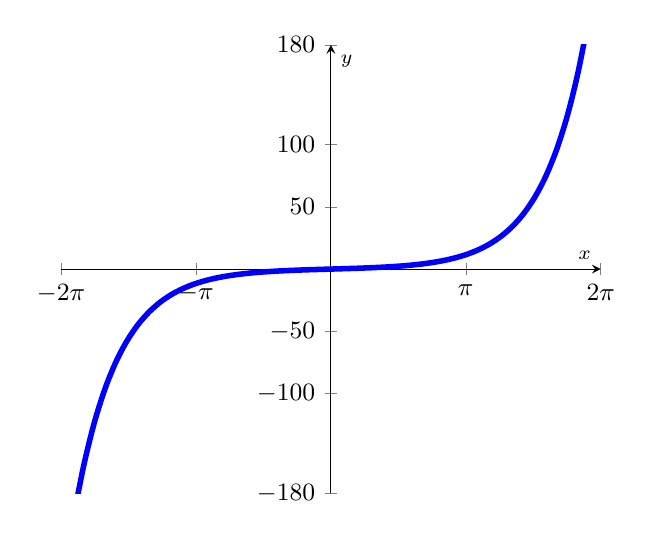
\begin{tikzpicture}[scale=1.0]
              \begin{axis}[axis lines=middle,xmin=-2*pi,xmax=2*pi,ymin=-180.0,ymax=180.0,
                xlabel=$\scriptstyle x$,
                ylabel=$\scriptstyle y$,
                xtick={-2*pi,-pi,0,pi,2*pi},
                xticklabels={$-2\pi$,$-\pi$,0,$\pi$,$2\pi$},
                ytick={-180,-100,-50,0,50,100,180},
                tick label style={font=\small}]
                \addplot[no marks,domain=-2*pi:2*pi,samples=50,smooth,line width=2pt,blue]{sinh(x)};
              \end{axis}
            \end{tikzpicture}
        \end{center}
\newpage
        \noindent \textbf{$\cosh(x)\ (ch(x))$ hatványsora és konvergencia tartománya}\\

        \noindent Írjuk fel a $\cosh x$ deriváltjait:

        \begin{itemize}
            \item $(\cosh x)^{(n)} = \sinh x$, ha $n$ páratlan, tehát $(\cosh 0)^{(2n+1)} = 0$
            \item $(\cosh x)^{(n)} = \cosh x$, ha $n$ páros, tehát $(\cosh 0)^{(2n)} = 1$
        \end{itemize}

        \noindent Így a hatványsor $\cosh x = \sum\limits_{n=0}^{\infty}\ddfrac{x^{2n}}{(2n)!}$\\

        \noindent A Lagrange-féle maradéktagból az approximációs hiba egy rögzített $x$ esetén:
        \[
            r_{2n}(x) \leq M \cdot \ddfrac{x^{2n}}{(2n)!}
        \]

        \noindent $M = max\Big\{\big|(\sinh x)^{(2n)}\big|\Big\} = \sinh x = const$. Így $r_{n} \to 0$, ha $n \to \infty$.\\

        \noindent Tehát a $\boldsymbol{\cosh(x) = \sum\limits_{n=0}^{\infty}\ddfrac{x^{2n}}{(2n)!}}$ bármely $x \in \mathbb{R}$ esetén.\\

      \begin{center}
          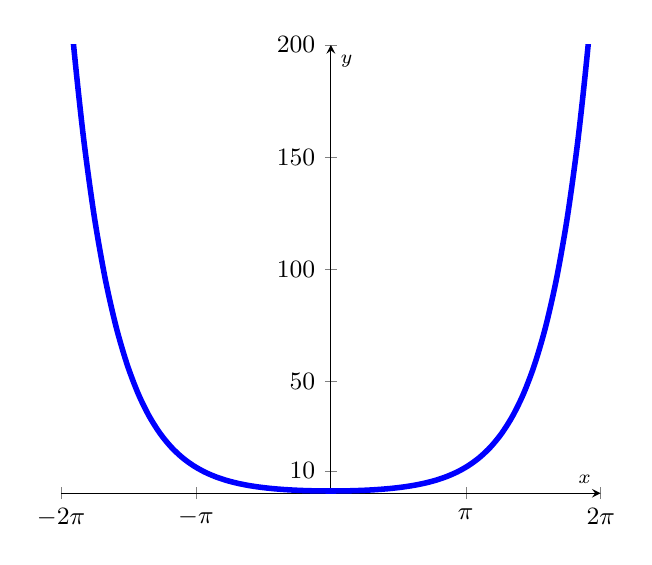
\begin{tikzpicture}[scale=1.0]
              \begin{axis}[axis lines=middle,xmin=-2*pi,xmax=2*pi,ymin=0.0,ymax=200.0,
                xlabel=$\scriptstyle x$,
                ylabel=$\scriptstyle y$,
                xtick={-2*pi,-pi,0,pi,2*pi},
                xticklabels={$-2\pi$,$-\pi$,0,$\pi$,$2\pi$},
                ytick={-200,-100,-150,-50,-10,0,10,50,100,150,200},
                tick label style={font=\small}]
                \addplot[no marks,domain=-2*pi:2*pi,samples=50,smooth,line width=2pt,blue]{cosh(x)};
              \end{axis}
            \end{tikzpicture}
        \end{center}
	
\end{document} 